\documentclass[11pt]{article}

\usepackage[margin=0.70in]{geometry}
\usepackage{amsmath,amssymb,graphicx,enumitem,booktabs,array}
\setlist[enumerate]{leftmargin=*,itemsep=8pt,topsep=4pt}

\begin{document}
\begin{center}\textbf{Optional CFD practice: payload trim before shape design}\end{center}

\section*{Purpose and submission}
This open-tool practice exercise prepares you for the in-class CFD interpretation practical. You may work alone or with others and may use the repository documentation, AI tools, notes, and any other resources. You are not being assessed on independent coding.

Week 1 holds the NACA 2412 geometry fixed and asks how incidence is selected to carry payload lift. Week 2 keeps that payload-trim idea, but asks whether changing geometry can lower cruise drag while preserving dash-condition margins.

\noindent\textbf{What JAX will do in Week 2.} JAX is a software tool that calculates a \emph{sensitivity}: if we make a very small change to camber or camber-crest location, how does calculated drag change? The code uses those sensitivities to choose the next geometry to try. JAX does not choose the requirements, judge safety, or replace engineering judgment.

You may submit the completed evidence sheet for small extra credit and feedback. Feedback addresses whether your claims are supported by your figures and data; it is not a grade for prose or authorship.

\section*{What to run}
Run \texttt{python course/build\_week1\_subcritical\_figures.py} from the repository root. It generates a NACA 2412 geometry, a lift/drag polar from an incidence sweep, and pressure plots at $\alpha=2^\circ$ and $4^\circ$. Do not alter the solver unless you wish to explore beyond the exercise.

\section*{Reference relations}
For this simplified screening exercise, the two-dimensional airfoil coefficients are treated as representative wing coefficients:
\[
 L=q_\infty S C_L,\qquad D=q_\infty S C_D,\qquad q_\infty=\tfrac12\rho_\infty V_\infty^2.
\]
For this practice study, hold $M_\infty=0.50$ fixed and vary only incidence $\alpha$. The payload target is approximately $C_L=0.75$. This is intentionally a subcritical study: no shock constraint or transonic design decision is part of Week 1.

\noindent\textbf{Model boundary.} This is a two-dimensional inviscid calculation. It is useful for identifying trends in pressure loading and lift, but it does not predict skin-friction drag, separation, three-dimensional effects, structural loads, or aircraft performance.

\newpage
\section*{A. Generate and inspect the incidence sweep}
The supplied script evaluates one NACA 2412 section over several angles of attack. Record the output values from your run. If you submit this page, attach the polar and the $\alpha=4^\circ$ surface-pressure plot.

\begin{center}
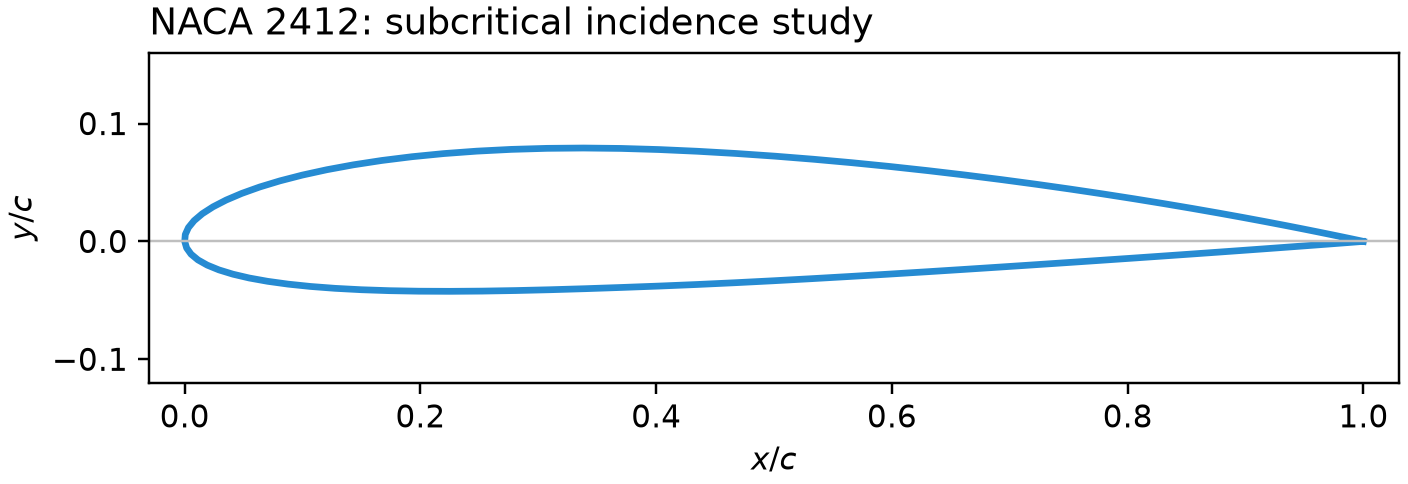
\includegraphics[width=.72\linewidth]{course/week1_figures/week1_geometry.png}
\end{center}

\begin{center}
\renewcommand{\arraystretch}{1.5}
\begin{tabular}{c|c|c|c|c|c|c}
Incidence $\alpha$ & $C_L$ & $C_D$ & Lift trend & Drag trend & Evidence used & Comment \\
\hline
$2^\circ$ & & & & & & \\
$4^\circ$ & & & & & & \\
$6^\circ$ & & & & & & \\
\end{tabular}
\end{center}

\begin{enumerate}
\item On the $\alpha=4^\circ$ pressure plot, label the upper and lower surfaces. Which surface has lower pressure over most of the chord?
\item From the polar, state what happens to $C_L$ when $\alpha$ increases. Why does this plot not prove a real-airfoil performance limit?
\item Name one real effect that this inviscid, two-dimensional calculation leaves out.
\end{enumerate}

\newpage
\section*{B. Bracket payload trim and connect to Week 2}
The Week 1 figures answer different questions: the polar summarizes integrated loads over incidence, while the $C_p$ curves show where the pressure loading comes from. This is a response study, not an optimization map.

\begin{center}
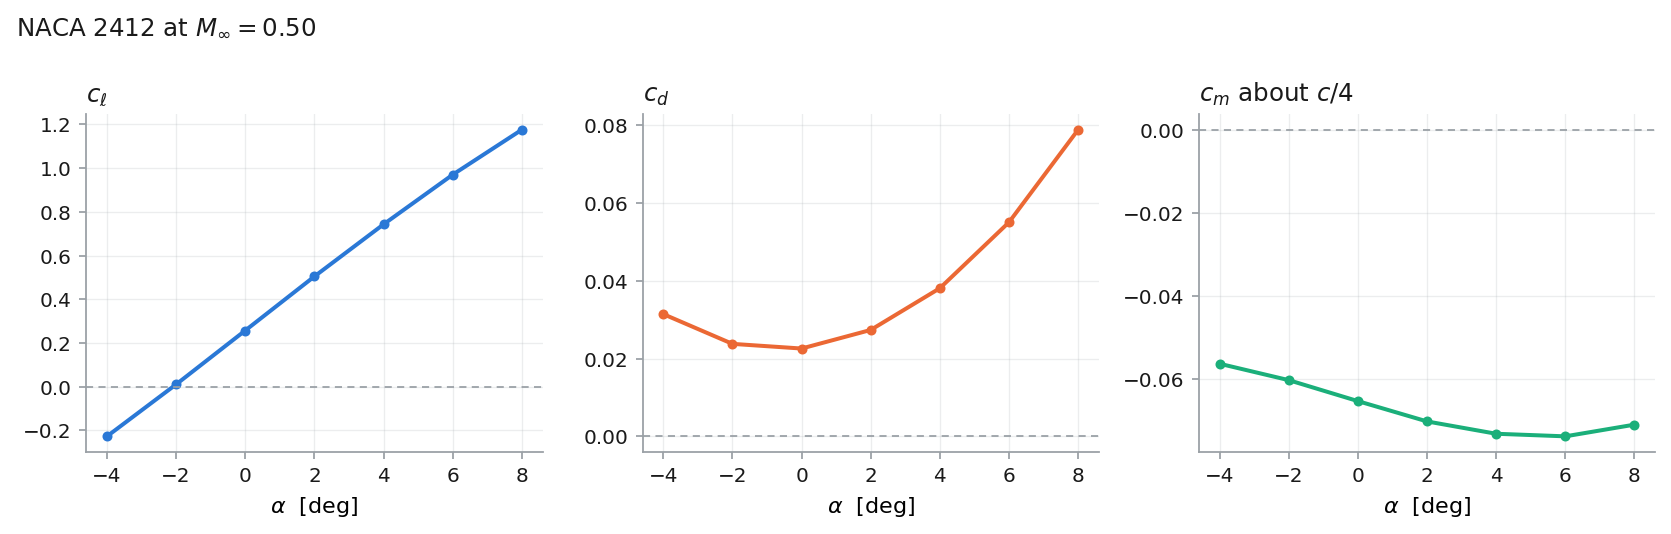
\includegraphics[width=.32\linewidth]{course/week1_figures/week1_polar.png}\hfill
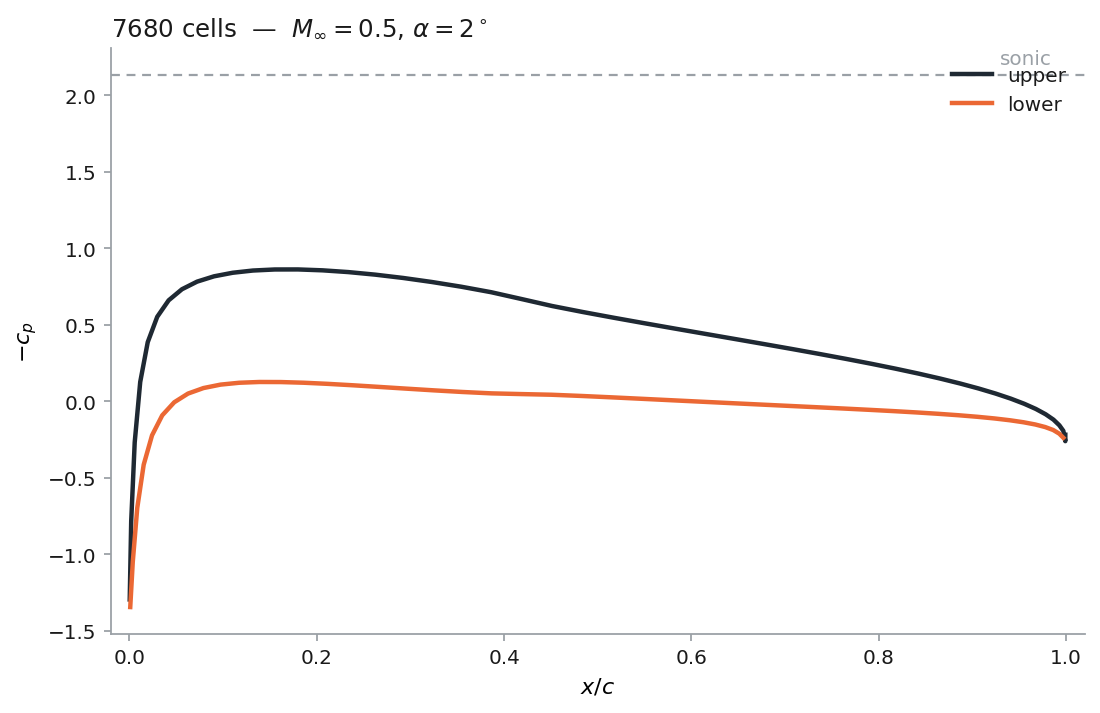
\includegraphics[width=.32\linewidth]{course/week1_figures/week1_cp_alpha2.png}\hfill
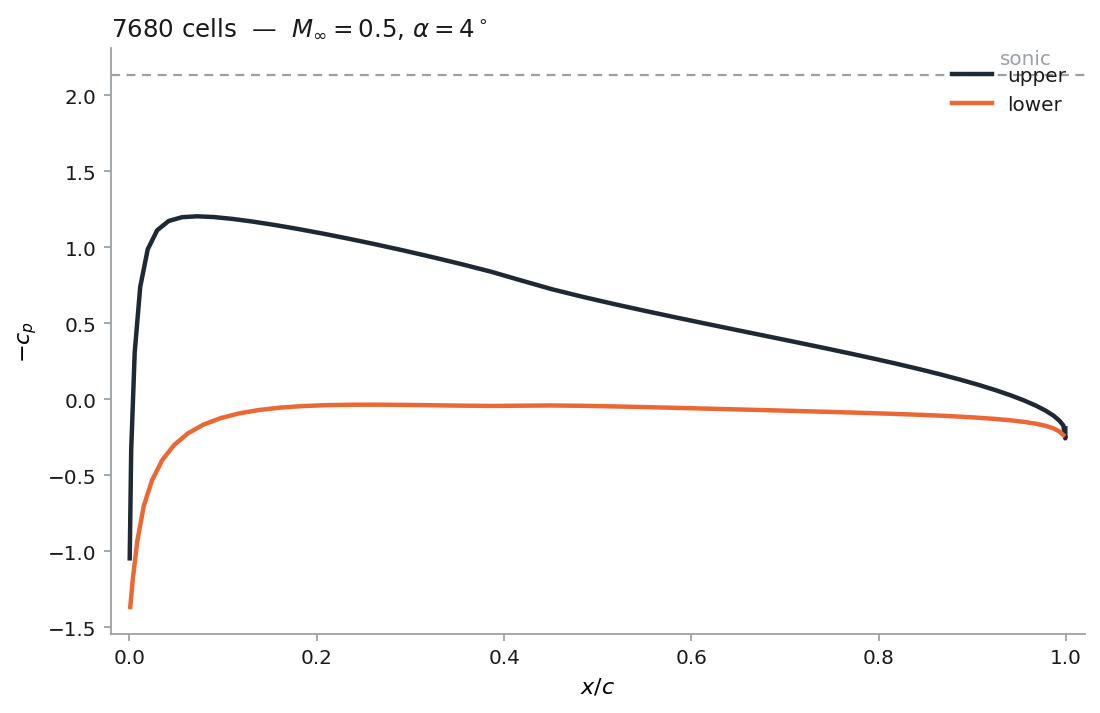
\includegraphics[width=.32\linewidth]{course/week1_figures/week1_cp_alpha4.png}
\end{center}

\noindent\textbf{Preliminary trim decision.} At this one subcritical operating condition, the payload target is $C_L\approx0.75$. Use the discrete sweep to bracket that target. A design operating condition must later be trimmed more precisely than this coarse sweep.
\[
C_L\approx0.75,\qquad C_D\leq0.050.
\]
\begin{enumerate}
\setcounter{enumi}{3}
\item Which two tested incidences surround $C_L=0.75$? Choose a first incidence to try. What incidence should be run next to reach $C_L=0.75$ more closely?
\item A polar gives total lift and drag. What information about the airfoil does it \emph{not} give?
\item Compare the $\alpha=2^\circ$ and $4^\circ$ $C_p$ curves. What changes on the upper surface, and how does that explain the larger lift?
\item In one sentence: what do you choose in Week 1, and what does JAX help change in Week 2?
\end{enumerate}

\newpage
\section*{Solution key (instructor review)}
\noindent Values read from the supplied polar are approximate. Award credit for equivalent, figure-supported statements.

\begin{enumerate}
\item[1.] The black curve is the upper surface and the orange curve is the lower surface. The upper surface has lower pressure over most of the chord: on the plot of $-C_p$, it has the larger value.
\item[2.] $C_L$ increases approximately linearly over the plotted incidence range: it is about $0.50$ at $2^\circ$, $0.74$ at $4^\circ$, and $0.97$ at $6^\circ$. This limited inviscid sweep does not establish a real-airfoil stall or performance limit.
\item[3.] Examples: the calculation cannot establish skin-friction drag, separation/stall, three-dimensional wing effects, structural loads, or full-aircraft performance.
\item[4.] The target is bracketed by $4^\circ$ ($C_L\approx0.74$, $C_D\approx0.027$) and $6^\circ$ ($C_L\approx0.97$, $C_D\approx0.055$). Use $4^\circ$ as the preliminary setting, then run an additional incidence between $4^\circ$ and $6^\circ$ (or a finer sweep) to trim exactly to $C_L=0.75$.
\item[5.] A polar contains integrated coefficients only. It cannot identify the chordwise location or surface responsible for a pressure-loading change; a $C_p(x/c)$ plot is needed.
\item[6.] At $4^\circ$, the upper-surface suction is stronger and the pressure difference between surfaces is larger. The greater area between the curves corresponds to the larger integrated lift in the polar.
\item[7.] Week 1 selects an \emph{operating incidence} for one fixed NACA 2412 section. Week 2 trims incidence for every geometry, then varies camber and crest position to trade cruise drag against dash Mach and moment margins.
\end{enumerate}
\end{document}

